%!TEX root = /Users/daniel/Documents/thesis/thesis.tex
\chapter[Detexify]{Detexify - \LaTeX-Symbolsuche als Webanwendung} % (fold)
\label{cha:detexify}

Bevor ich auf die technischen Details von Detexify eingehe sollten Sie, lieber Leser, sich kurz mit dem Programm vertraut gemacht haben. Die Beschreibungen sind dann viel verständlicher. Die Benutzung von Detexify sollte selbsterklärend sein. Sollten Sie doch Schwierigkeiten haben finden Sie in \ref{man:benutzerhandbuch} ein kurzes Benutzerhandbuch. Sie können auf Detexify mit einem modernen Browser\footnote{Aktuelle Versionen von Firefox, Chrome, Safari und Opera \TODO IE testen.} unter der Adresse \url{http://detexify.kirelabs.org} zugreifen.

Die folgenden Abschnitte enthalten neben der Beschreibung der Funktionalität von Detexify außerdem Hinweise zur Implementierung.

\section{Architektur} % (fold)
\label{sec:architektur}

Bei jeder Anwendung muss man sich, bevor sie geschrieben wird, entscheiden, wie die Anwendung zur Verfügung gestellt werden soll. Daraus resultieren weitere Entscheidungen, wie z.B. die Wahl der Programmiersprache und der Datenformate.

Detexify wurde als Webanwendung implementiert. Dies hat die folgenden Vorteile:

\begin{itemize}
  \item \textbf{Plattformunabhängigkeit:} Heutzutage ist ein Webbrowser auf jedem Computer verfügbar. Um Detexify verwenden zu können wird nur ein moderner\footnotemark[1] Webbrowser benötigt.
  \item \textbf{Zentrale Wartung:} Fehlerbehebungen und Verbesserungen sind zentral anwendbar und stehen jedem Benutzer beim nächsten Besuch der Anwendung sofort zur Verfügung.
  \item \textbf{Zentrale Trainingsdaten:} Die Trainingsdaten sind zentral in einer Datenbank gespeichert. Das Training der Klassifizierers wird von den Nutzern selbst durchgeführt (siehe auch \ref{sec:crowdsourcing}).
\end{itemize}

Dabei besteht Detexify aus zwei lose gekoppelten Komponenten und zwar der Webanwendung und dem Klassifizierungsserver (Server). Lose Kopplung heisst dabei, dass lediglich ein Interface definiert ist, wie die Webanwendung mit dem Server zu kommunizieren hat. (\TODO loose coupling in der Literatur) Das Interface ist als \ac{REST}-Interface spezifiziert. Die beiden Komponenten kommunizieren also über \ac{HTTP}. Abbildung~\ref{fig:architecture} zeigt die Architektur schematisch.

\begin{figure}
  \centering 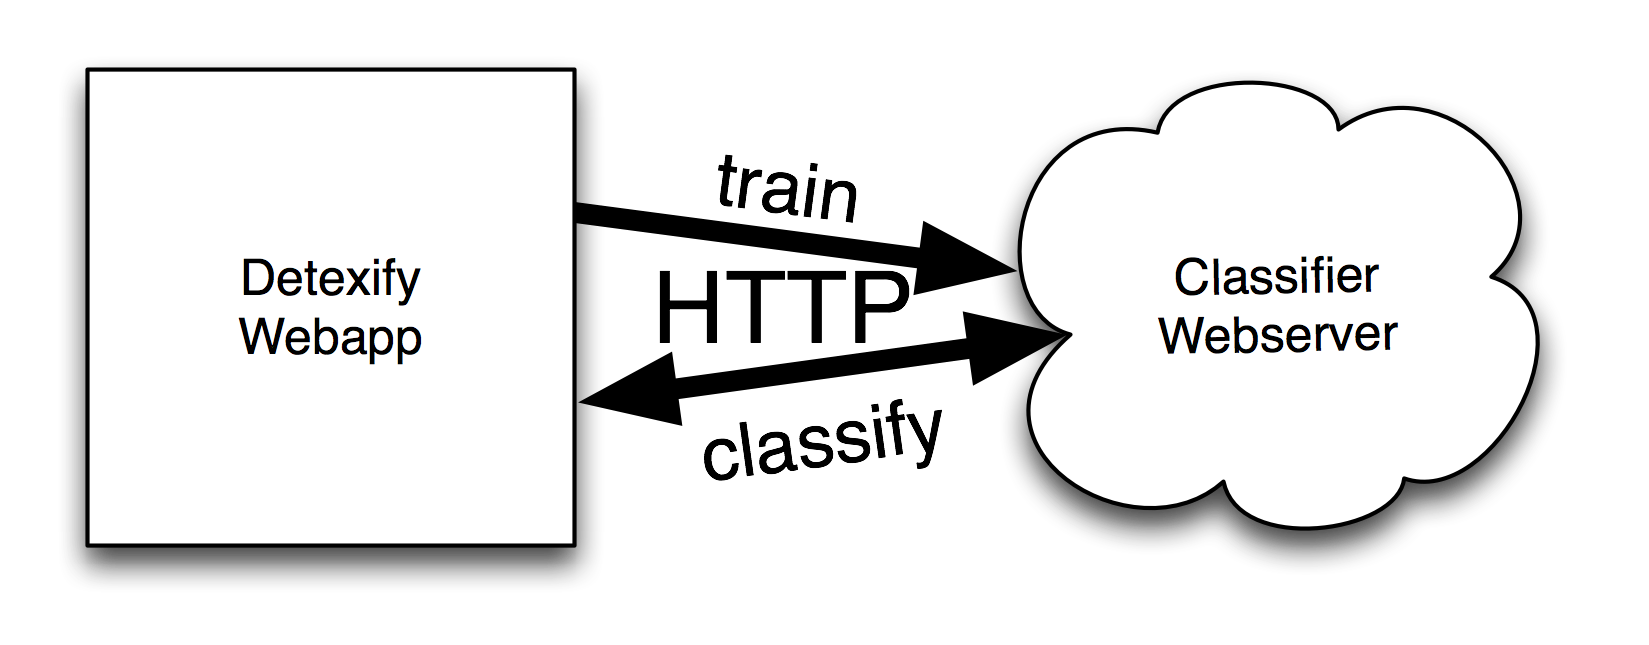
\includegraphics{figures/architecture.pdf}
  \caption{Detexify Architektur}
  \label{fig:architecture}
\end{figure}

\section{Webanwendung} % (fold)
\label{sec:webanwendung}

% section webapp (end)

Die Webanwendung stellt das Benutzerinterface von Detexify dar. Sie wird über einen Browser bedient. Es gibt zwei Sichten (jeweils durch statische \ac{HTML}-Seiten und Javascript realisiert.) Die erste Sicht ermöglicht die Symbolsuche und die zweite Sicht bietet eine Symboltabelle aller in Detexify registrierten \LaTeX-Symbole. In dieser können die Symbole auch trainiert werden.

\subsection{Symbolsuche} % (fold)
\label{sub:symbolsuche}

Die Symbolsuche ist das Zentrum der Anwendung. Sie ist das Werkzeug, das dem \LaTeX-Entwickler das Leben vereinfachen soll. Abbildung~\ref{fig:symbolsuche} zeigt einen Screenshot eines Browsers mit geöffneter Symbolsuche.

Auf der Seite der Webanwendung ist dafür eine Zeichenfläche implementiert. Auf dieser können mit der Maus (oder einem Grafiktablett) Striche gemalt werden, und nach jedem beendeten Strich wird per AJAX\footnote{Siehe \ref{sec:ajax}} eine Erkennungsanfrage an den Server gesendet. Die Symbole werden dann anhand der vom Server ermittelten Rangfolge aufgelistet wie in Abbildung~\ref{fig:symbolsuche} zu sehen. Die Kommunikation erfolgt wie in \ref{sec:server} erwähnt über das Datenformat \ac{JSON}. Die Interaktion ist mithilfe von Javascript gelöst. Die Zeichenfläche basiert auf der \ac{SVG}-Technologie.

\begin{figure}
  \centering 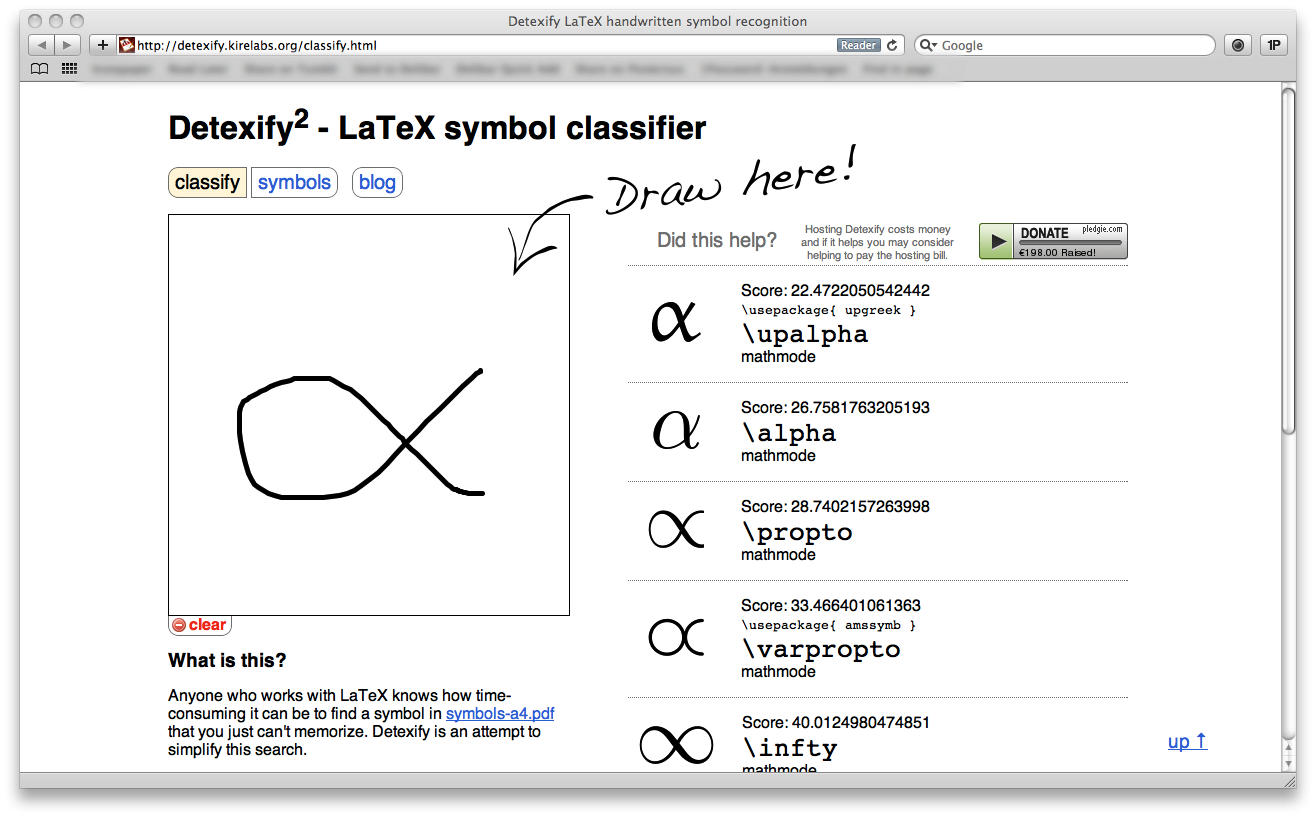
\includegraphics[width=\textwidth]{figures/interface-classify.png}
  \caption{Symbolsuche}
  \label{fig:symbolsuche}
\end{figure}

% subsection symbolsuche (end)

\subsection{Symboltabelle} % (fold)
\label{sub:symboltabelle}

Einerseits bietet die Symboltabelle einen Überblick über die in Detexify registrierten und damit über die Symbolsuche auffindbaren Symbole. Andererseits bietet die Symboltabelle durch ihre Sortierungs- und Filtermöglichkeiten von sich aus gute Möglichkeiten zur Symbolsuche, sollte die eigentliche Symbolsuche aus irgendwelchen Gründen versagen. Außerdem können in der Symboltabelle geziehlt einzelne Symbole trainiert werden. Die Funktionalität der Symboltabelle ist im Detail in \ref{man:symboltabelle} beschrieben. Die verwendeten Technologien sind sind identisch mit den bei der Symbolsuche verwendeten.
 Abbildung~\ref{fig:symboltabelle} zeigt einen Screenshot eines Browsers mit geöffneter Symboltabelle.

\begin{figure}
  \centering 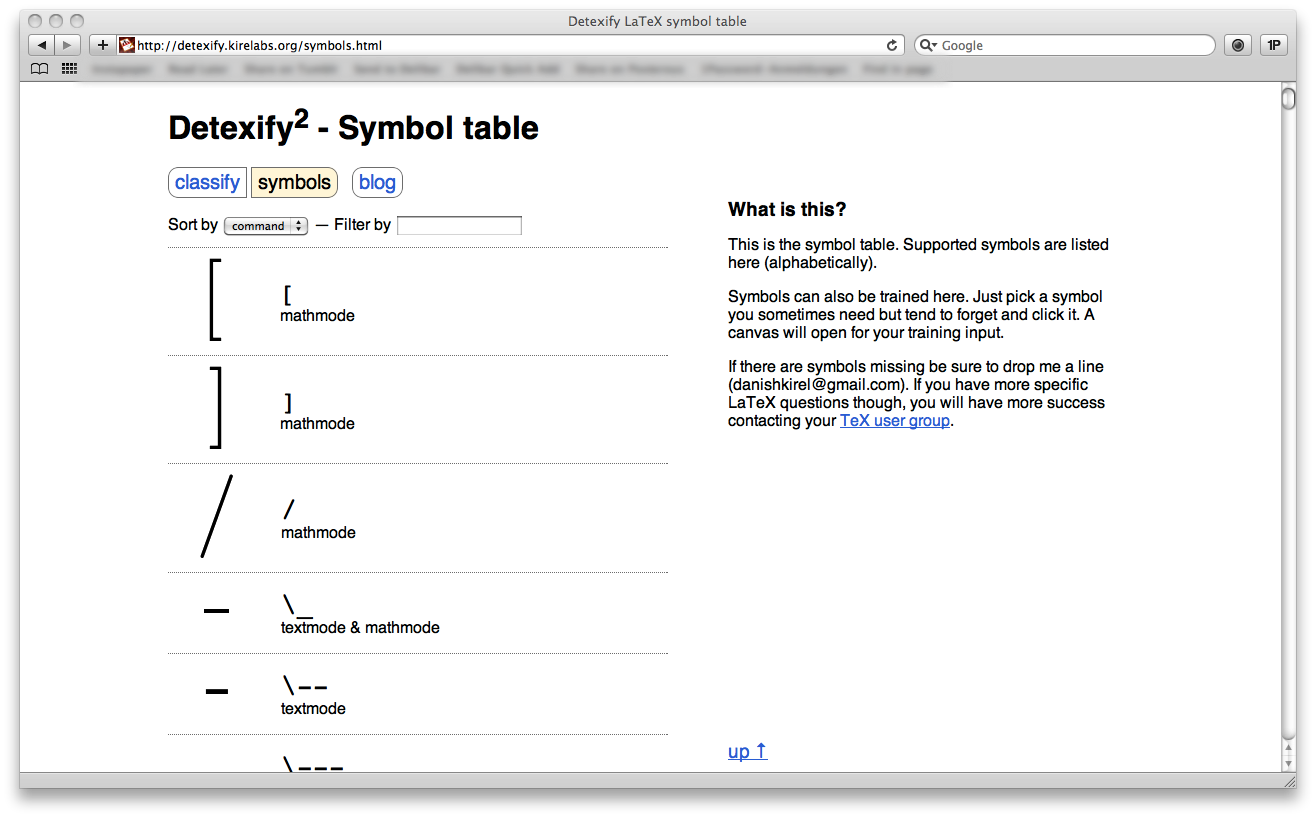
\includegraphics[width=\textwidth]{figures/interface-symbol-table.png}
  \caption{Symboltabelle}
  \label{fig:symboltabelle}
\end{figure}

% subsection symboltabelle (end)


\section{Server} % (fold)
\label{sec:server}

Der Server übernimmt die Mustererkennung. An ihn können im wesentlichen zwei verschiedene Anfragen gestellt werden. Die erste davon ist das Training einer Symbolklasse. Die zweite ist die Klassifizierung von unbekannten Daten. Es gibt noch eine dritte Anfrage, die aber lediglich zur Identifizierung und Statusermittlung der Serverimplementierung dient.

Da der Server die eigentliche Arbeit verrichtet läuft er auf einem leistungsstarken Rechner. \TODO Wieso keine Parallelisierung, wo wir doch eh schon in der Wolke sind...

Das \ac{REST}-Interface\footnote{Genauere Erklärungen zu \ac{REST} findet der Leser in \ref{sec:rest}} sieht folgendermaßen aus:

\subsection{REST-Interface} % (fold)
\label{sub:rest_interface}

\subsubsection{Training}

Um eine Symbolklasse zu trainieren müssen dem Server der Bezeichner der Klasse und die Trainingsdaten übergeben werden. Der Bezeichner ist dabei Teil der \ac{URL} und die Trainingsdaten werden als \ac{JSON}\footnote{Siehe \ref{sec:json}}-String im \ac{HTTP}-Request-Body übertragen.

\begin{lstlisting}[caption={Anfrage}]
  POST /train/{id}
  application/json
  [[{"x":12.3, "y":4.56, "t":7890},...],...]
\end{lstlisting}
\begin{lstlisting}[caption={Antwort}]
  200 OK
\end{lstlisting}
\begin{lstlisting}[caption={Antwort im Fehlerfall}]
  422 Unprocessable Entity
  application/json
  { "error" : "error message" }
\end{lstlisting}

\subsubsection{Erkennung}
\label{subsub:erkennung}

Zur Erkennung werden die unbekannten Daten als \ac{JSON}-String an den Server übertragen. Dies geschieht wie beim Training im \ac{HTTP}-Request-Body. Als Antwort erhält die Webanwendung eine \ac{JSON}-kodierte Liste von Klassenbezeichnern und einer zugehörigen Wertung. Je kleiner die Wertung, desto wahrscheinlicher die zugehörige Klasse.

\begin{lstlisting}[caption={Anfrage}]
  POST /classify
  application/json
  [[{"x":12.3, "y":4.56, "t":7890},...],...]
\end{lstlisting}
\begin{lstlisting}[caption={Antwort}]
  200 OK
  application/json
  [{ "id" : "key", "score": 1.234}, ...]
\end{lstlisting}
\begin{lstlisting}[caption={Antwort im Fehlerfall}]
  422 Unprocessable Entity
  application/json
  { "error" : "error message" }
\end{lstlisting}

\subsubsection{Serverstatus}

Durch die lose Kopplung durch das hier definierte Interface lässt sich der Server leicht austauschen\footnote{Tatsächlich existieren Serverimplementierungen in drei verschiedenen Programmiersprachen.} und um die verwendete Serverimplementierung identifizieren zu können gibt es noch eine dritte Anfrage, die aber zur Funktionalität des Servers nichts beiträgt.

\begin{lstlisting}[caption={Anfrage}]
GET /
\end{lstlisting}
\begin{lstlisting}[caption={Antwort}]
200 OK
application/json
{ 
  "server" : "server string to identify implementation",
  "version" : "version string e.g. 1.0"
}
\end{lstlisting}
  
% subsection rest_interface (end)

% section server (end)


\section{Crowdsourcing des Trainings} % (fold)
\label{sec:crowdsourcing}

Wie in \ref{sub:symboltabelle} erwähnt bietet Detexify den Nutzern ein Interface um das Training durchzuführen. Tatsächlich habe ich nie ein initiales Training vorgenommen. Der Plan war von Anfang an, das Training vollständig den Nutzern zu überlassen. So eine Vorgehensweise nennt man Schwarmauslagerung (Crowdsourcing) \TODO Literatur. Die Überlegung war dabei die Folgende: Wenn die Nutzer von guten Trainingsdaten durch bessere Erkennungsraten profitieren, sind sie auch bereit ein wenig Arbeit zu investieren, damit einige von ihnen ausgewählte Symbole leicht gefunden werden. Durch die Streuung der Auswahl der Nutzer wird eine große Menge an Symbolen in kurzer Zeit auf einen guten Trainingsstand gebracht. \TODO Welche anderen Beispiele für erfolgreiche Schwarmauslagerung gibt es? Delicious z.B.?

Diese Tatik ist voll aufgegangen. Als Detexify am 11. Juli 2009 online ging, war die Idee völlig neu. Eine \LaTeX-Symbolsuche in dieser Form hatte zu diesem Zeitpunkt noch niemand gesehen, daher verbreiteten sich Links zu Detexify in Windeseile über soziale Netze wie \href{http://twitter.com}{Twitter}, \href{http://facebook.com}{Facebook} und \href{http://delicious.com}{Delicious} aber auch über Newsportale wie \href{http://reddit.com}{Reddit} und \href{http://news.ycombinator.com}{Hacker News} und am 14. Juli 2009 erreichte Detexify seinen Spitzenwert von über 10.000 Besuchern an einem Tag. Erst gegen Ende Juli 2009 normalisierten sich die Besucherzahlen. Bis zu diesem Zeitpunkt hatten die Nutzer bereits mehrere Tausend Trainingsbeispiele gespendet. Zur Zeit liegt die Anzahl an Trainingsbeispielen bei über 130.000 für 977 Symbole.

\TODO Schwarmauslagerung, Schwarmintelligenz etc... da gibts doch sicher Literatur. Ich kann ja nicht nur schwafeln.

\TODO http://delicious.com/popular/latex <- Platz 3 am 25.7.2010 <- kann ich das noch irgendwie unterbringen?

% section crowd_sourcing (end)

% chapter detexify (end)
